\chapter{Work Completed}
	\section{Data Accumulation}
		We used dataset created during a Deepfake Image Detection and Reconstruction
		Challenge. Two datasets of real face images were used: CelebA and FFHQ. Various
		Deepfake images were generated using architectures such as StarGAN, GDWCT,
		AttGAN, StyleGAN, and StyleGAN2. Specifically, CelebA images were manipulated
		using pre-trained models available on GitHub for StarGAN, GDWCT, and AttGAN.
		Images from StyleGAN and StyleGAN2 created through FFHQ were obtained. A sample of real and fake images are shown below:

	\begin{figure}[hbt!]
		\centering
		\begin{minipage}{0.45\textwidth}
				\centering
				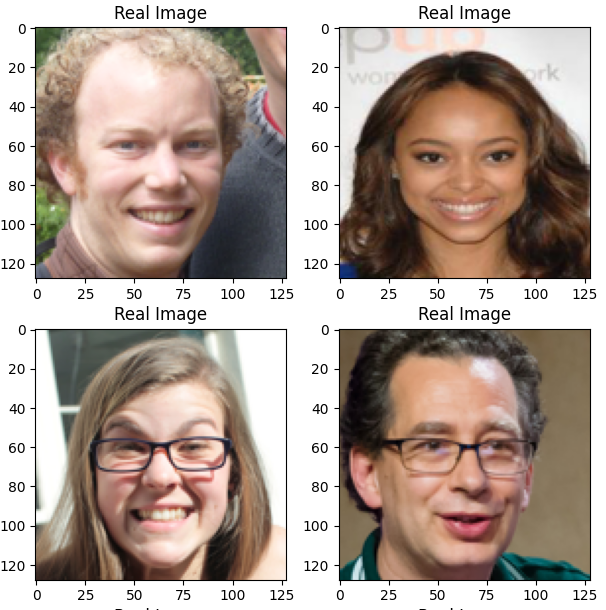
\includegraphics[width=0.95\linewidth]{./img/real sample.png}
				\caption{Real Images}
		\end{minipage}
		\hfill
		\begin{minipage}{0.45\textwidth}
				\centering
				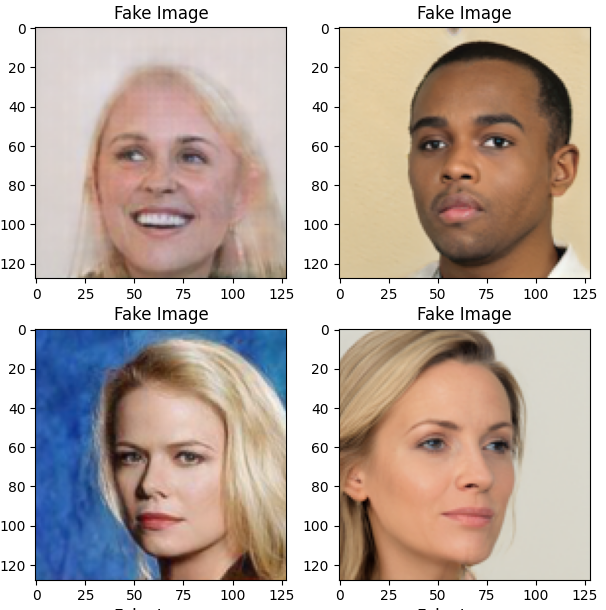
\includegraphics[width=0.95\linewidth]{./img/fake sample.png}
				\caption{Fake Images}
		\end{minipage}
	\end{figure}

	\section{Data Preprocessing}
	\subsection{Data Augmentation}
		To balance our dataset, we augmented our images to achieve a total of 25000 images for each category. For the 5000 fake images, we applied four different transformations, resulting in 20000 augmented fake images. For the real images, we randomly selected and transformed 3750 images, generating 15000 augmented real images. Various transformations, such as rotation, compression, scaling, and mirroring, were implemented. A sample of each transformation is shown below:

	\begin{figure}[hbt!]
		\centering
		\begin{minipage}{0.45\textwidth}
				\centering
				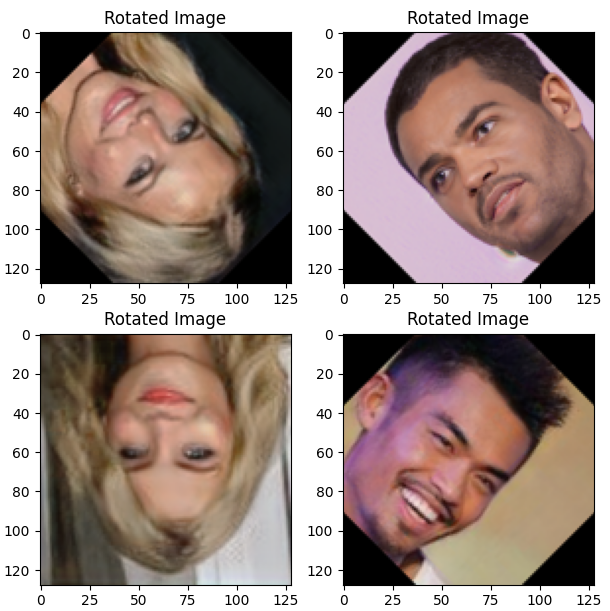
\includegraphics[width=0.95\linewidth]{./img/rotated.png}
				\caption{Rotated Images}
		\end{minipage}
		\hfill
		\begin{minipage}{0.45\textwidth}
				\centering
				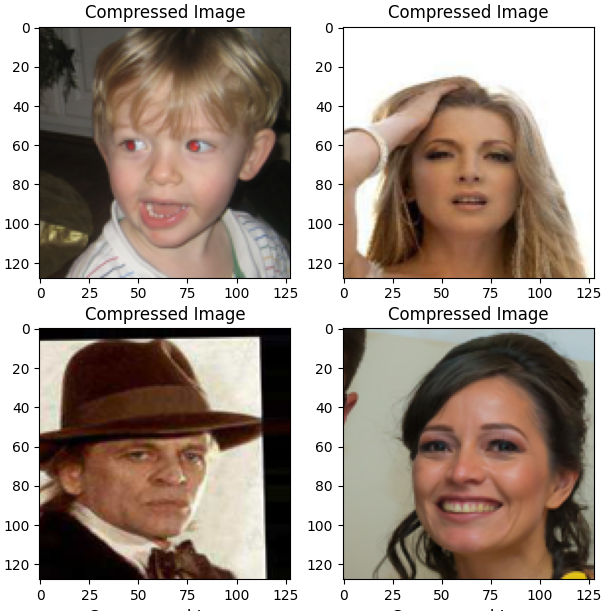
\includegraphics[width=0.95\linewidth]{./img/compressed.png}
				\caption{Compressed Images}
		\end{minipage}

		\vspace{0.5cm} % Add some vertical space between the two rows of images

		\begin{minipage}{0.45\textwidth}
				\centering
				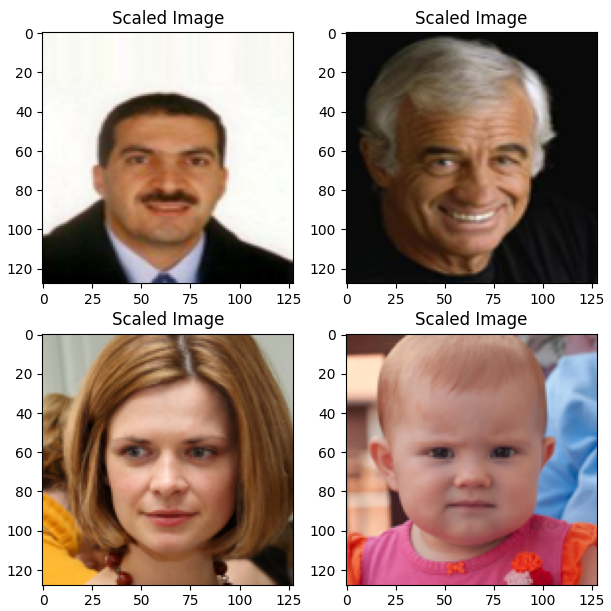
\includegraphics[width=0.95\linewidth]{./img/scaled.png}
				\caption{Scaled Image}
		\end{minipage}
		\hfill
		\begin{minipage}{0.45\textwidth}
				\centering
				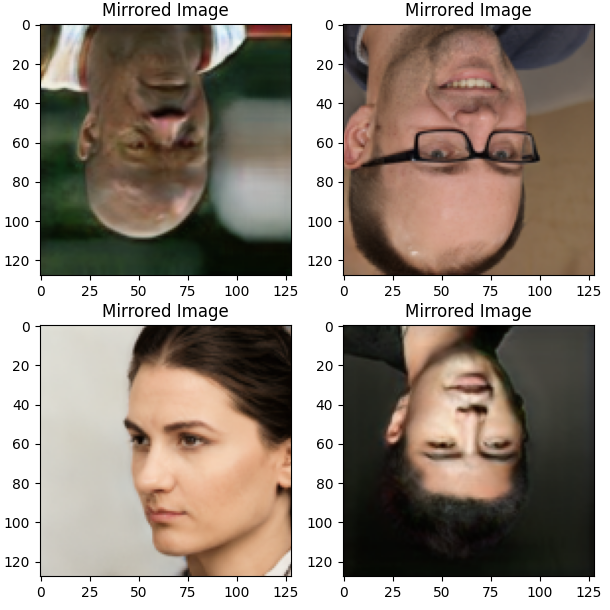
\includegraphics[width=0.95\linewidth]{./img/mirrored.png}
				\caption{Mirrored Images}
		\end{minipage}
	\end{figure}

	\subsection{Data Normalization}
	First, we computed the mean and standard deviation of the entire dataset, which consists of both the original dataset and the augmented dataset. The normalization process was then applied using the following formula:
	\begin{equation}
	x = \frac{x - \mu}{\sigma}
	\end{equation}
	where \(x\) represents the pixel values of each image pixel.
	
	This approach standardizes the features to have a mean of 0 and a standard deviation of 1. This standardization is crucial because certain machine learning algorithms are sensitive to the scale of the input features.

	\subsection{Data Splitting}
	We partitioned our dataset into a training set, comprising 80\% of the dataset, and a validation set, consisting of 20\% of the dataset. This division ensures that the model has an ample amount of data for learning, while also offering a subset of the data to assess the model's performance.

	\section{Setting Parameters}
	\begin{itemize}
		\item \textbf{Number of epochs : 50} \\
			The number of epochs refers to the number of times the complete training dataset is passed through the network during the training process. Each epoch consists of one forward pass (input to output) and one backward pass (error calculation and weight updates) for all the training samples.
		\item \textbf{Loss function : Cross-Entropy} \\
			Loss function is a method of evaluating how well your algorithm models your dataset. Cross-entropy loss measures the difference between a deep learning classification model's discovered and predicted probability distributions.

			The cross-entropy between two probability distributions, such as q from p, can be stated formally as
			
			\begin{equation}
				H(p, q) = -\sum_{x \in \mathcal{X}} p(x) \log q(x)
			\end{equation}

			Where
			\begin{itemize}
				\item H is the cross-entropy function
				\item p may be the target distribution
				\item q is the approximation of the target distribution.
			\end{itemize} 

		\item \textbf{Learning rate : 0.001} \\
			The learning rate is a hyperparameter that determines the step size at which an optimization algorithm.
		\item \textbf{Optimizer : Adam} \\
			An optimizer  is an algorithm used to update the parameters (weights and biases) of a model during training in order to minimize the loss function. 
			Adam (short for Adaptive Moment Estimation) is a popular optimization algorithm known for its robustness, efficiency, and ease of use. It often converges faster and performs better than traditional optimization algorithms.
			It adapts the learning rate for each parameter individually based on the past gradients and squared gradients making it well suited for training models.
	\end{itemize}

	\section{Model Training}
		We tested various customs models as well as pre-trained models like VGG16\_bn, ResNet50, ResNet101, and many more. During this process, We came to a conclusion that ResNet9 was performing much better than other models. So, We are using ResNet9 architecture for further training and implementation process.
		
		The model begins with an input layer configured to accept images with dimensions of 128x128 pixels and three color channels (RGB). Following this, the first convolutional layer is applied, utilizing 64 filters of size 3x3. Each filter convolves across the input image, extracting various features such as edges and textures. Batch normalization is then performed to normalize the activations of the convolutional layer, enhancing training stability. Subsequently, a rectified linear unit (ReLU) activation function is applied, introducing non-linearity to the network by replacing negative values with zeros.

		Moving forward, the second convolutional layer processes the output of the previous layer, applying 128 filters of size 3x3. Again, batch normalization and ReLU activation follow suit. Additionally, a max-pooling layer with a 2x2 window and a stride of 2 downsamples the feature maps, reducing spatial dimensions and computational complexity.

		Next, a residual block, inspired by the ResNet architecture, is introduced. This block comprises two convolutional layers, each followed by batch normalization and ReLU activation. The output of these layers is added to the output of the second convolutional layer, fostering better gradient flow during training and mitigating the vanishing gradient problem.

		Continuing, convolutional layer 3 is applied, employing 256 filters of size 3x3. Batch normalization and ReLU activation are again utilized for feature map normalization and non-linearity introduction, respectively. Another max-pooling layer further reduces spatial dimensions.

		Subsequently, convolutional layer 4 is employed, employing 512 filters of size 3x3. Similar to prior layers, batch normalization and ReLU activation are applied. Following this, another residual block, akin to ResNet architecture, is employed, aiding in feature extraction and gradient flow enhancement.

		Finally, a max-pooling layer with a 4x4 window reduces the spatial dimensions further. The resultant feature maps are then flattened into a 1D vector, which undergoes dropout regularization with a rate of 0.2, randomly deactivating 20\% of neurons during training to prevent overfitting. Lastly, a fully connected layer with two units, likely indicative of binary classification, applies a softmax activation function to generate class probabilities.
	\newpage
	\begin{figure}[hbt!]
		\center{
			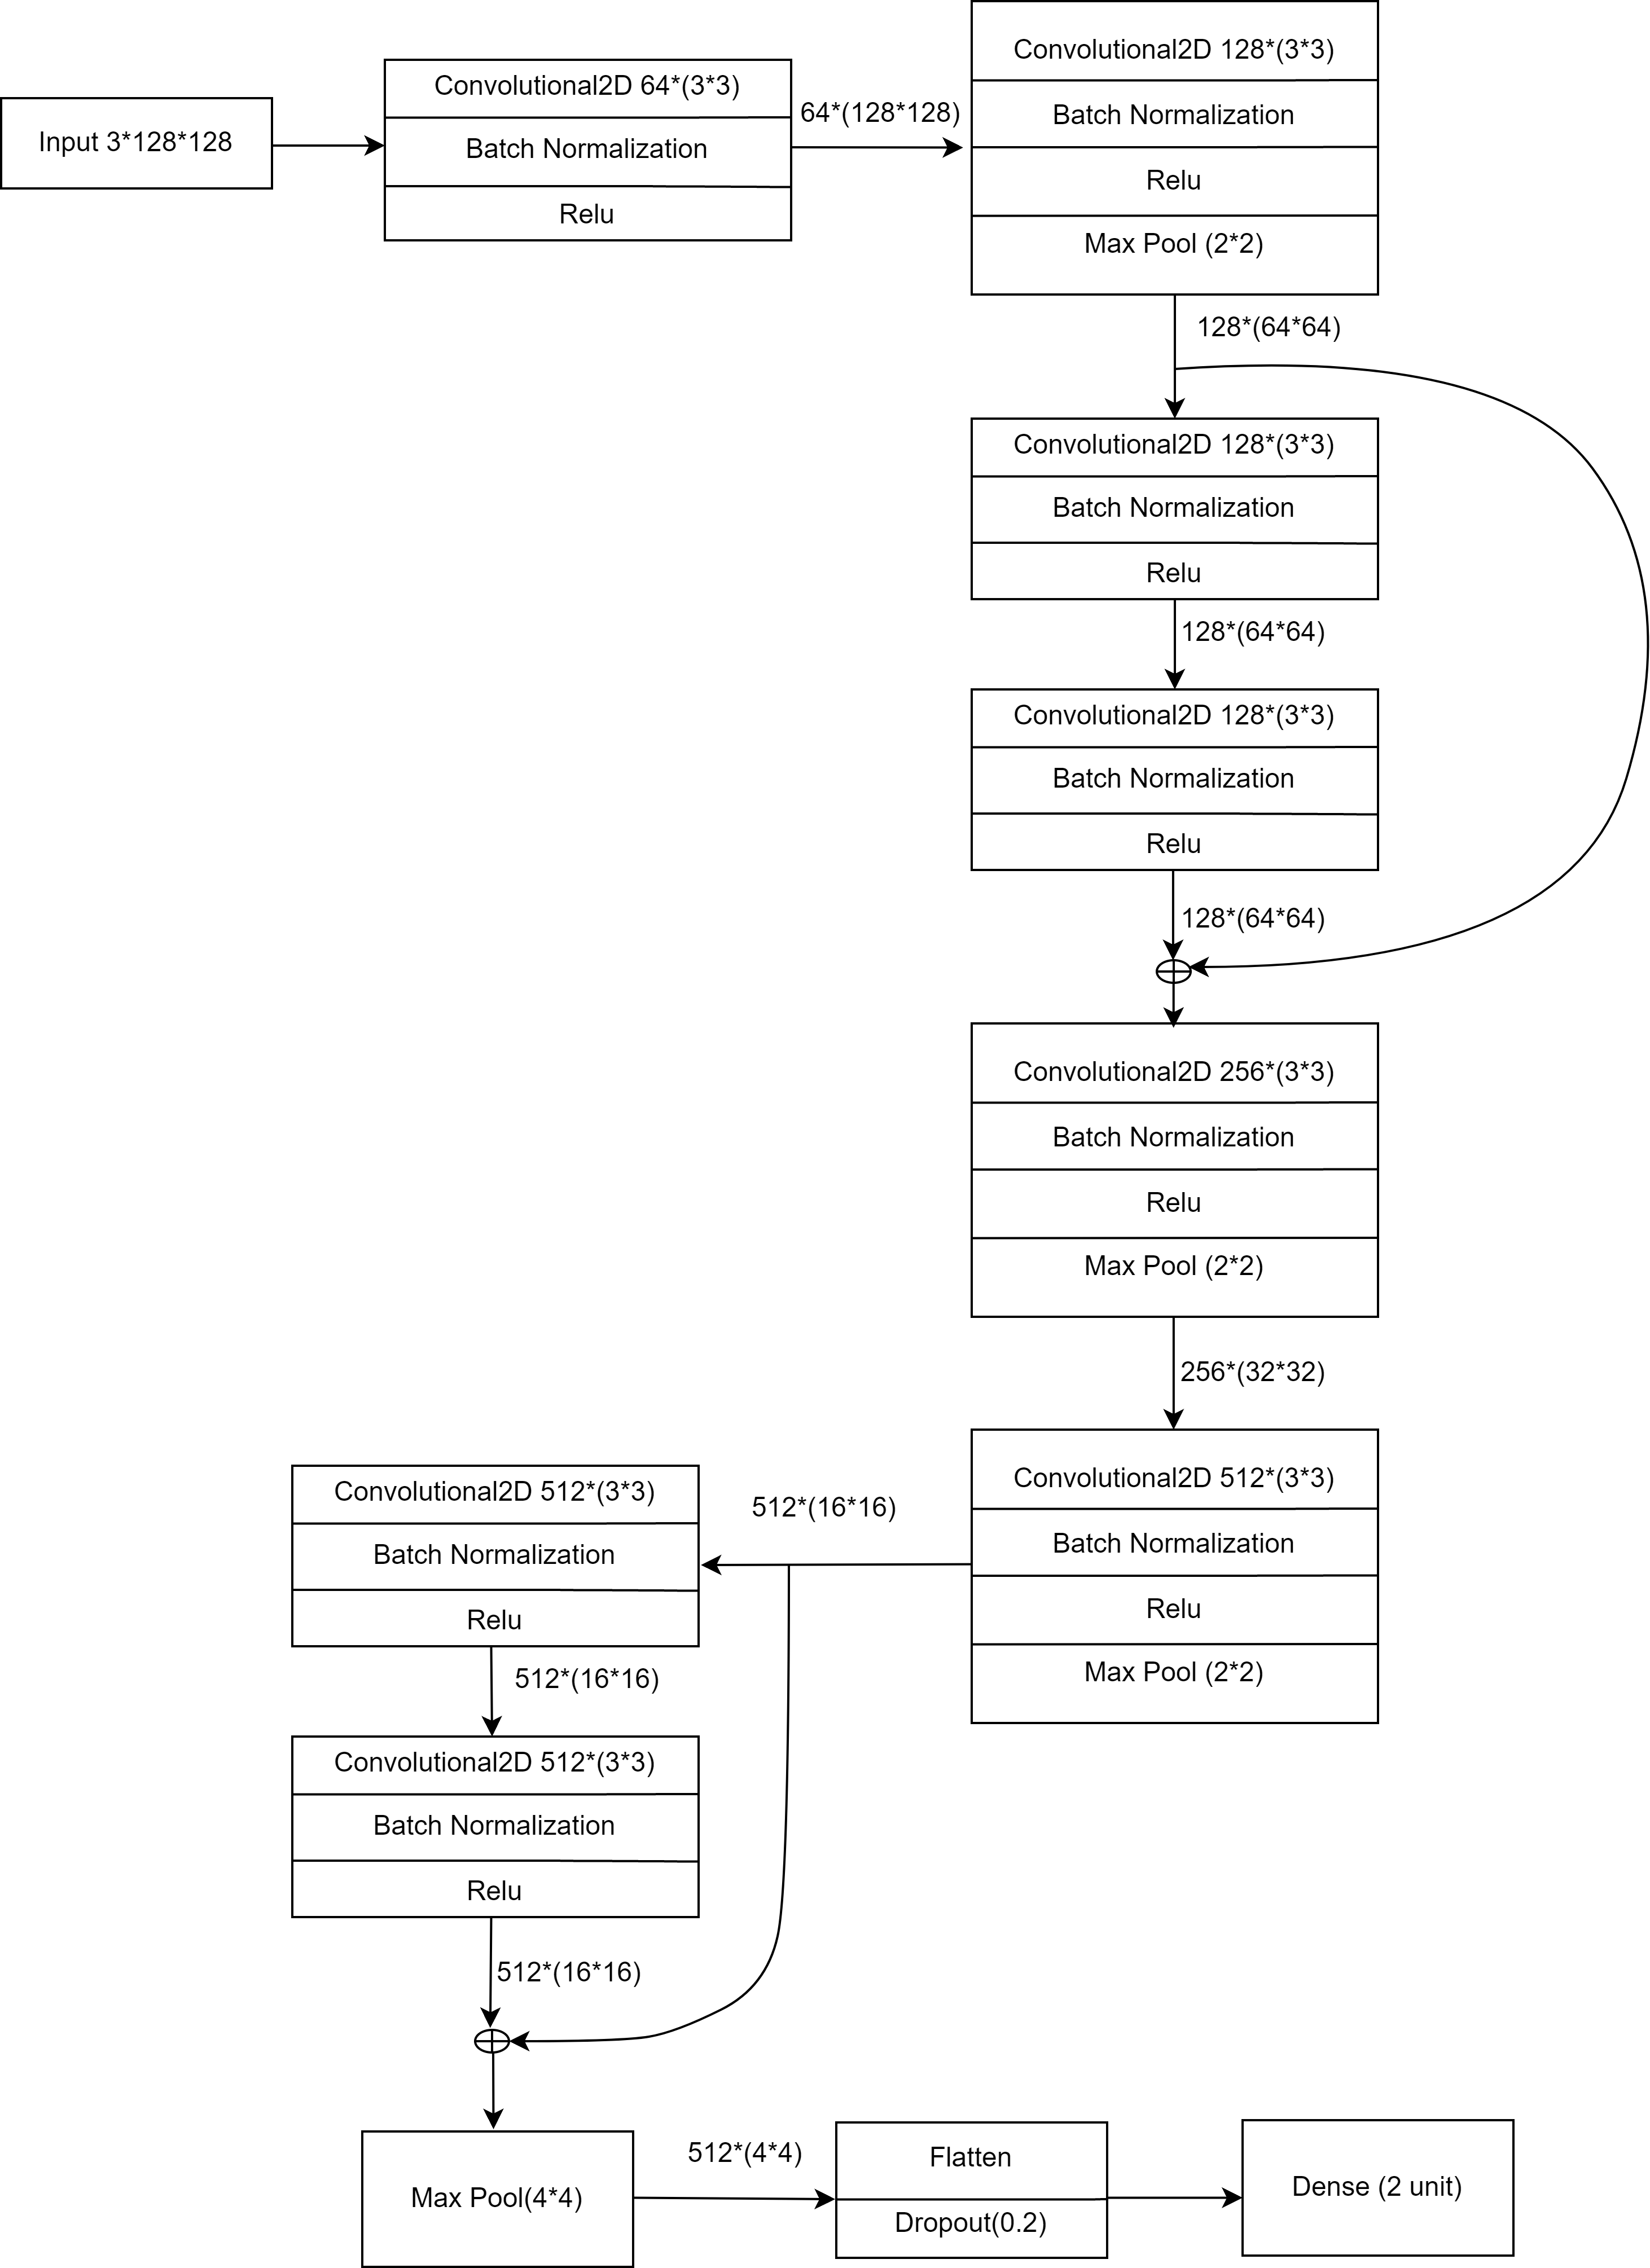
\includegraphics[width=0.68\textheight]{./img/layers.png}
			\caption{Architecture of ResNet9 Model}
		}
	\end{figure}

	\section{Model Evaluation}
	\begin{figure}[hbt!]
		\center{
			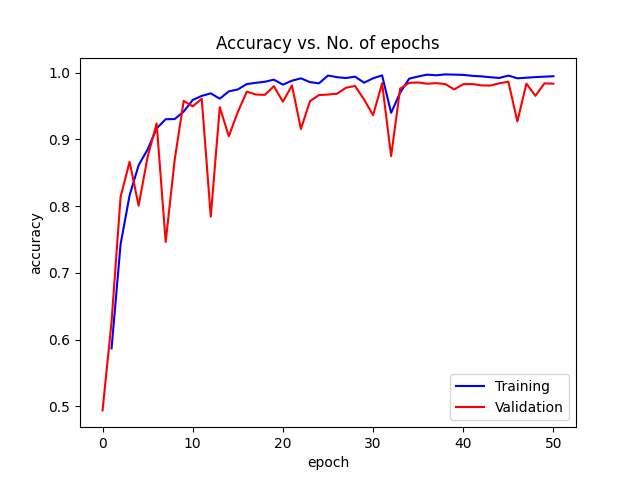
\includegraphics[width=0.8\textwidth]{./img/resnet9accuracy.png}
			\caption{Accuracy vs. No. of epochs }
		}
	\end{figure}
	\begin{figure}[hbt!]
		\center{
			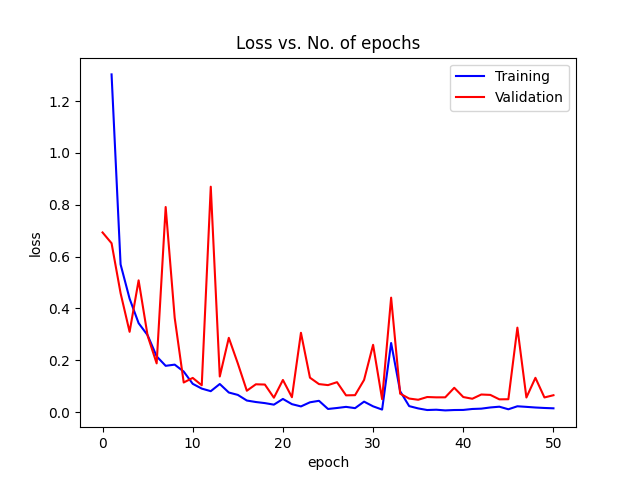
\includegraphics[width=0.8\textwidth]{./img/resnet9losses.png}
			\caption{Loss vs. No. of epochs}
		}
	\end{figure}

	\subsection*{Testing Results}
	We used the test dataset given on the DeepFake Detection Challenge\cite{jimaging8100263} to test our models performance.
	Testing dataset consist of 5000 fake images and 2000 real images.
	\vspace{1pt}
	\begin{figure}[hbt!]
		\center{
			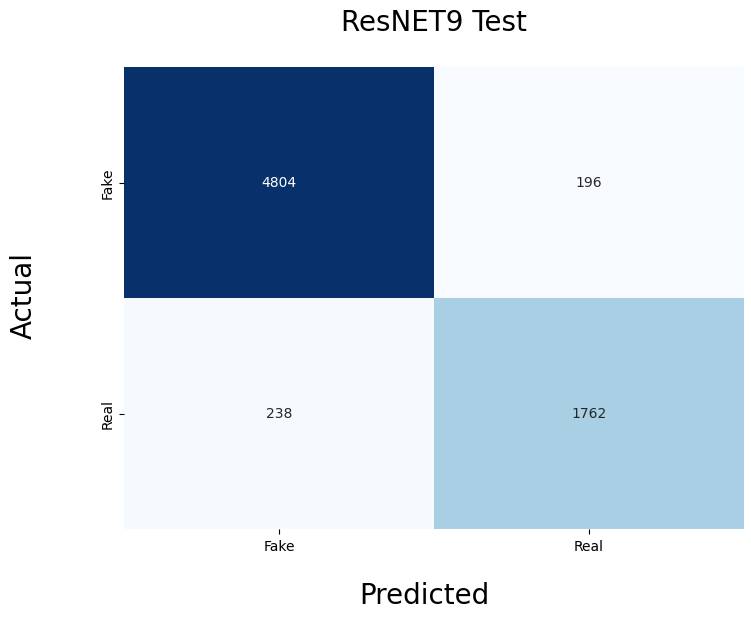
\includegraphics[width=1\textwidth]{./img/confusion_matrix.png}
			\caption{Confusion Matrix}
		}
	\end{figure}

	% \newpage
	\begin{enumerate}
		\item Accuracy
		\begin{equation}
				\text{Accuracy} = \frac{\text{TP} + \text{TN}}{\text{TP} + \text{TN} + \text{FP} + \text{FN}}
		\end{equation}
		\item Precision
		\begin{equation}
			% \begin{flalign}
				\text{Precision} = \frac{\text{TP}}{\text{TP} + \text{FP}}
			% \end{flalign}
		\end{equation}
		\item Recall
		\begin{equation}
			\text{Recall} = \frac{\text{TP}}{\text{TP} + \text{FN}}
		\end{equation}
		\item F1 Score
		\begin{equation}
			\text{F1 Score} = 2 \times \frac{\text{Precision} \times \text{Recall}}{\text{Precision} + \text{Recall}}
		\end{equation}

		where
		TP = True Positive,
		TN = True Negative,
		FP = False Positive,
		FN = False Negative
		\item Reciever Operating Characteristic (ROC) Curve
			\begin{figure}[hbt!]
				\center{
					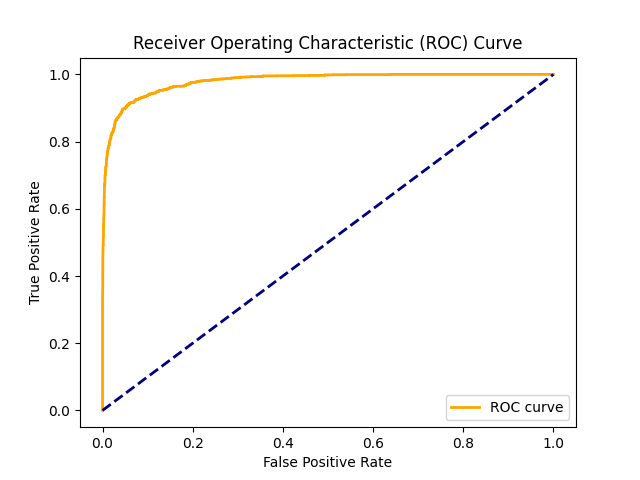
\includegraphics[width=1\textwidth]{./img/ROC.png}
					\caption{Reciever Operating Characteristic (ROC) Curve}
				}
			\end{figure}

			\textbf{Area Under ROC Curve = 0.9209}

\begin{table}[h!]
		\centering
		\begin{tabular}{lccccc}
		\multicolumn{6}{c}{\textbf{}} \\ 
		\multicolumn{6}{c}{\textbf{}} \\ 
		\textbf{} & \textbf{Accuracy} & \textbf{Precision} & \textbf{Recall} & \textbf{F1-score} & \textbf{Support} \\
		\textbf{Fake}  & 96.08\% & 0.952 & 0.960 & 0.955 & 5000 \\
		\textbf{Real} & 88.10\%  & 0.899 & 0.881 & 0.889 & 2000 \\
		\textbf{Macro Avg} & 92.09\% & 0.925 & 0.920 & 0.922 & 7000 \\
		\textbf{Weighted Avg} & 93.80\% & 0.936 & 0.938 & 0.937 &7000 \\ 
		\multicolumn{6}{c}{\textbf{}} \\
		\multicolumn{6}{c}{\textbf{}} \\
		\end{tabular}
		\caption{Performance Table}
		\end{table}
\end{enumerate}

\newpage
\section{User Interface}

\begin{figure}[hbt!]
	\center{
		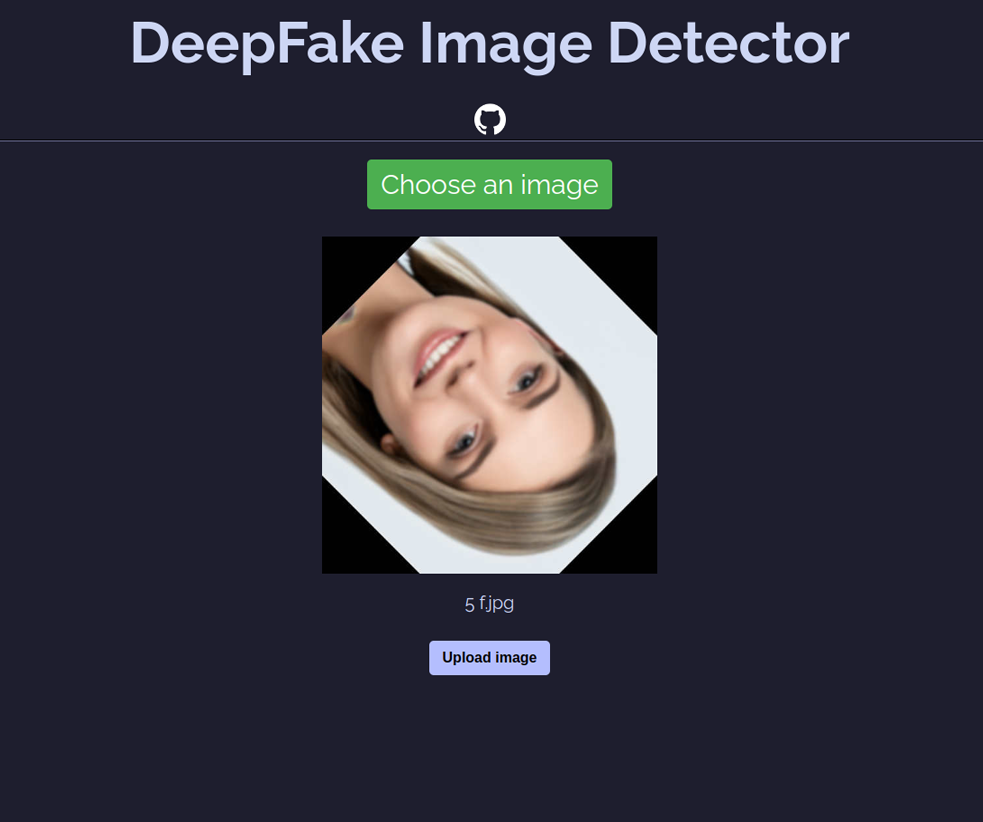
\includegraphics[width=0.66\textwidth]{./img/UI1.png}
		\caption{Demonstration of model detecting real image}
	}
\end{figure}
\begin{figure}[hbt!]
	\center{
		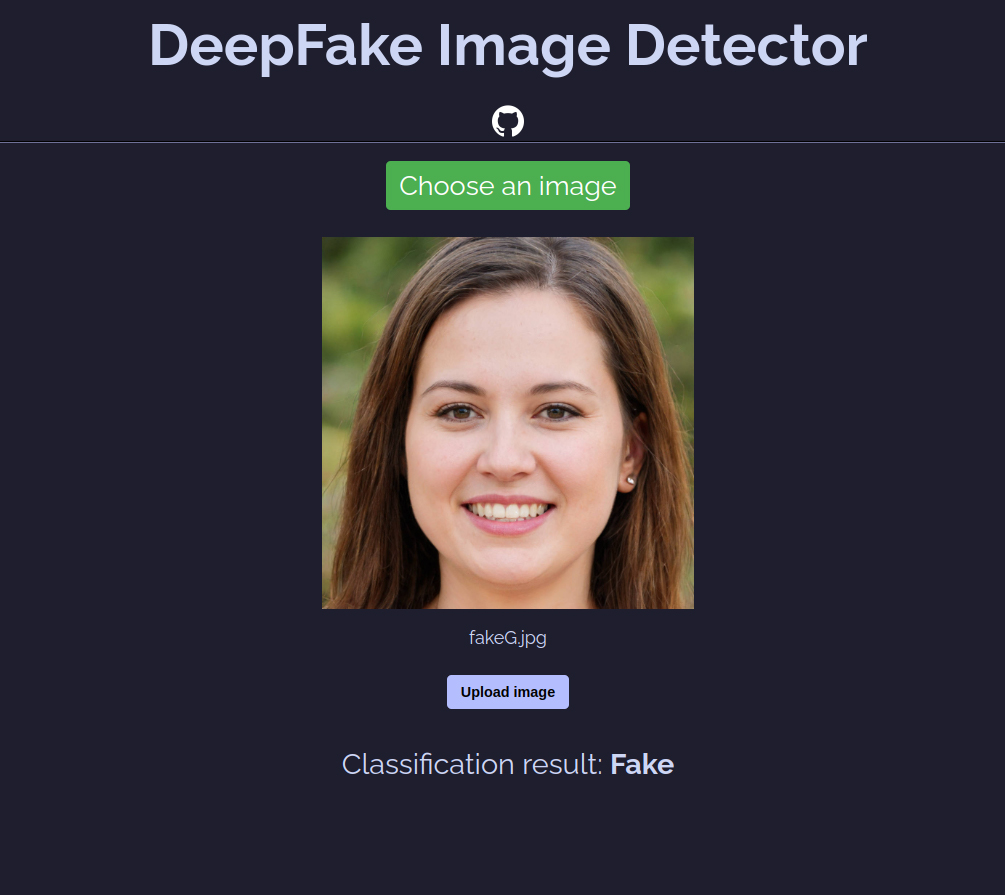
\includegraphics[width=0.66\textwidth]{./img/UI2.jpg}
		\caption{Demonstration of model detecting fake image}
	}
\end{figure}